% ============================================================
%  LLM-Based Antipattern Detection in UML Use Case Models
%  Conference paper — generic article template
% ============================================================
\documentclass[12pt, a4paper]{article}

% ── Packages ──────────────────────────────────────────────────────────────────
\usepackage[T1]{fontenc}
\usepackage[utf8]{inputenc}
\usepackage{lmodern}
\usepackage[margin=2.5cm]{geometry}
\usepackage{microtype}
\usepackage{hyperref}
\usepackage{booktabs}
\usepackage{array}
\usepackage{graphicx}
\usepackage{xcolor}
\usepackage{listings}
\usepackage{caption}
\usepackage{subcaption}
\usepackage{amsmath}
\usepackage{enumitem}
\usepackage{parskip}
\usepackage{fancyhdr}
\usepackage[numbers,square,sort&compress]{natbib}
\usepackage{upquote}
\usepackage{float}

% Fix bibliography indentation: natbib calls \NAT@bibsetnum with the
% thebibliography argument (empty "" from apalike.bbl), computing \labelwidth
% from \@biblabel{} = "[]" — too narrow for actual number labels like [19].
% Redefine \NAT@bibsetnum to always use \@biblabel{99} for correct alignment.
% (Cannot patch \@bibsetup directly: natbib reassigns it via \let inside
%  \AtBeginDocument{\NAT@set@cites}, which runs after any preamble override.)
\makeatletter
\renewcommand\NAT@bibsetnum[1]{%
  \settowidth\labelwidth{\@biblabel{99}}%
  \setlength{\leftmargin}{\labelwidth}\addtolength{\leftmargin}{\labelsep}%
  \setlength{\itemsep}{\bibsep}\setlength{\parsep}{\z@}%
  \ifNAT@openbib
    \addtolength{\leftmargin}{\bibindent}%
    \setlength{\itemindent}{-\bibindent}%
    \setlength{\listparindent}{\itemindent}%
    \setlength{\parsep}{0pt}%
  \fi
}
\makeatother

% ── Colours ───────────────────────────────────────────────────────────────────
\definecolor{codeblue}{rgb}{0.13,0.29,0.53}
\definecolor{codegray}{rgb}{0.45,0.45,0.45}
\definecolor{codegreen}{rgb}{0.0,0.45,0.18}
\definecolor{codered}{rgb}{0.65,0.08,0.18}

% ── Listings style ────────────────────────────────────────────────────────────
\lstset{
  basicstyle=\ttfamily\footnotesize,
  keywordstyle=\color{codeblue}\bfseries,
  commentstyle=\color{codegray}\itshape,
  stringstyle=\color{codegreen},
  numberstyle=\tiny\color{codegray},
  numbers=left,
  numbersep=8pt,
  frame=single,
  rulecolor=\color{black!20},
  backgroundcolor=\color{black!3},
  breaklines=true,
  breakatwhitespace=true,
  tabsize=2,
  captionpos=b,
  showstringspaces=false,
}

% ── JSON language for listings ────────────────────────────────────────────────
\lstdefinelanguage{json}{
  morestring=[b]",
  stringstyle=\color{codegreen},
  morekeywords={true,false,null},
  keywordstyle=\color{codeblue}\bfseries,
}

% ── Header / footer ───────────────────────────────────────────────────────────
\pagestyle{fancy}
\fancyhf{}
\fancyhead[L]{\small\textit{LLM-Based Antipattern Detection in UML Use Case Models}}
\fancyhead[R]{\small\thepage}
\renewcommand{\headrulewidth}{0.4pt}

% ── Metadata ──────────────────────────────────────────────────────────────────
\hypersetup{
  pdftitle={LLM-Based Antipattern Detection in UML Use Case Models},
  pdfauthor={},
  colorlinks=true,
  linkcolor=codeblue,
  citecolor=codeblue,
  urlcolor=codeblue,
}

% ==============================================================================
\begin{document}

% ── Title block ───────────────────────────────────────────────────────────────
\title{%
  \textbf{LLM-Based Antipattern Detection in UML Use Case Models:\\[4pt]
  A Synthetic Data Generation and Fine-Tuning Approach}
}
\author{%
  Yasser Khan\\
  \small Department of Electrical Engineering and Computer Science\\
  \small Florida Atlantic University, Florida, USA\\
  \small \texttt{khany2026@fau.edu}
  \and
  Mohamed El-Attar\\
  \small College of Technological Innovation\\
  \small Zayed University, Abu Dhabi, United Arab Emirates\\
  \small \texttt{Mohamed.El-Attar@zu.ac.ae}
}
\date{}
\maketitle
\thispagestyle{fancy}

% ── Abstract ──────────────────────────────────────────────────────────────────
\begin{abstract}
Antipatterns in UML use case models degrade software design quality and
impede communication between stakeholders, yet their detection has received
comparatively little automated support.  We present a complete pipeline for
fine-tuning an LLM to detect the \emph{Functional Decomposition
via} \texttt{<<include>>} \emph{relationship} antipattern in PlantUML use
case diagrams.  The pipeline uses Claude Opus, a frontier LLM,
to synthesize 194 labeled diagram pairs (each consisting of an antipattern
version and its correctly refactored counterpart) across a diverse set of
application domains.  Qwen2.5-Coder-3B-Instruct, a compact LLM, is then
fine-tuned on this dataset using Low-Rank Adaptation (LoRA), achieving
91.0\% detection accuracy and an instance-level recall of 0.85 on a held-out, domain-stratified test set.  The paper details the full pipeline from synthetic data generation to fine-tuning and evaluation.
\end{abstract}

\noindent\textbf{Keywords:} UML, use case diagrams, antipattern detection,
LLM, fine-tuning, synthetic data, PlantUML, LoRA.

\vspace{1em}
\hrule
\vspace{1em}

% ==============================================================================
\section{Introduction}
\label{sec:intro}

Unified Modeling Language (UML) use case diagrams are a primary artifact in
requirements engineering.  They describe the functional scope of a
system in terms of actors, use cases, and the relationships between them
(\texttt{<<include>>}, \texttt{<<extend>>}, and generalisation).  Despite their
conceptual simplicity, practitioners regularly introduce structural antipatterns that reduce
diagram clarity, misrepresent system behavior, or create maintenance
obstacles~\cite{lilly1999pitfalls,anda2001quality}.

One particularly common antipattern is \emph{Functional Decomposition via
the include relationship} (FD-include)~\cite{elattar2006matching,elattar2010improving}: a use case is decomposed into several
inclusion use cases that have no direct association with any actor and
provide no observable result of their own.  Detecting such instances requires
understanding both the syntactic structure of the diagram and the semantic
intent of the include relationship, a task that benefits from natural language
reasoning as well as structural analysis.

Existing approaches to antipattern detection in UML rely primarily on
model-checking rules, OCL constraints, or pattern-matching heuristics
\cite{gogolla2003validation,ballis2008rule,fourati2011metric}.  These methods are brittle when diagrams
do not conform to an expected representation, and they cannot generalize to
novel antipattern types without expert-authored rules.  Recent advances in
large language models (LLMs) offer an alternative: models trained on
sufficiently representative examples can generalize structural reasoning to
unseen diagrams.

However, assembling labeled training data for UML antipatterns is expensive
and scarce in practice.  Published datasets of annotated use case diagrams are
small and domain-narrow.  We address this bottleneck with a synthetic
data generation approach: we use Claude Opus, a state-of-the-art LLM, as a
controlled diagram author to produce a large, diverse, and precisely
labeled set of diagram pairs.  This data is then used to fine-tune
Qwen2.5-Coder-3B-Instruct, a compact open-source LLM suitable for
deployment in resource-constrained settings.

This paper presents a prompt-engineering framework
that instructs an LLM to produce syntactically valid, structurally diverse,
and correctly labeled antipattern/refactored PlantUML diagram pairs, together
with a structured dataset of 388 annotated training samples spanning 194
distinct application domains with 1--5 antipattern instances per diagram.
Building on this data, we fine-tune a 3B-parameter LLM that achieves 91.0\%
detection accuracy on domain-held-out test samples.

The remainder of this paper is structured as follows.
Section~\ref{sec:background} reviews relevant background.
Section~\ref{sec:pipeline} describes the data generation pipeline.
Section~\ref{sec:dataset} characterizes the resulting dataset.
Section~\ref{sec:finetuning} details the fine-tuning configuration.
Section~\ref{sec:evaluation} presents evaluation results.
Section~\ref{sec:discussion} discusses findings and limitations.
Section~\ref{sec:related} surveys related work.
Section~\ref{sec:conclusion} concludes.

% ==============================================================================
\section{Background}
\label{sec:background}

\subsection{UML Use Case Diagrams and Antipatterns}

A UML use case diagram represents the functional requirements of a system as
a set of use cases (ellipses) associated with one or more actors.  Three
relationship types express dependencies between use cases: the
\texttt{<<include>>} relationship indicates that the base use case always
incorporates the behavior of the inclusion use case; \texttt{<<extend>>}
represents optional behavior that may be inserted at an extension point; and
generalisation captures inheritance between actors or between use cases,
indicating that one element is a specialized form of another.

Antipatterns in use case models are recurring modeling mistakes that violate
the intended semantics of these elements~\cite{elattar2010improving}.
This work focuses on FD-include, where a use case is divided into several
inclusion use cases that are not directly associated with any actor.
Offering no observable result to a user, they represent internal sub-steps
rather than independent services.
The correct refactoring merges these inclusions back into the base use case.
Concretely, an inclusion use case participates in an FD-include instance
if and only if: (i) it is included by exactly one base use case; (ii) it has
no direct actor association; (iii) it neither includes nor extends any other
use case; (iv) it is not extended by any other use case; and (v) it is not
involved in any generalisation.

\subsection{LLMs for Code and Diagram Generation}

LLMs have demonstrated strong capabilities in generating
structured text conforming to domain-specific syntaxes, including source
code, configuration files, and markup languages.  PlantUML is a text-based
diagram description language; its grammar is sufficiently regular that
frontier models can produce syntactically valid diagrams with minimal
additional scaffolding.
This has been demonstrated in security modeling contexts: ChatGPT-5 has
been shown to generate misuse case diagrams directly in PlantUML from
textual security requirements~\cite{enase26}, and ChatGPT has been
evaluated for generating STRIDE data flow diagrams, with findings covering
syntactic correctness, semantic accuracy, and trust-boundary
placement~\cite{alsayegh2026stride}.


Low-Rank Adaptation (LoRA)~\cite{hu2022lora} is a parameter-efficient
fine-tuning technique that injects trainable low-rank matrices into each
weight matrix of a frozen pre-trained model.  With rank $r \ll d$, where $d$
is the dimension of the weight matrix, LoRA reduces the number of trainable parameters
by orders of magnitude while preserving performance comparable to full
fine-tuning.

% ==============================================================================
\section{Data Generation Pipeline}
\label{sec:pipeline}

\subsection{Pipeline Overview}

The pipeline takes two inputs.  The first is an antipattern specification
that names the antipatterns to be instantiated, providing a natural-language
description and a refactoring strategy for each.  The second is a pool of
194 application domains spanning everyday (e.g.\ Banking System, Online
Store), moderately common (e.g.\ Tutoring Marketplace, Crowdfunding
Platform), and niche domains (e.g.\ Irrigation Control System, Funeral
Service Management System), ensuring the model sees a wide
range of domain vocabularies.  These inputs drive three pipeline stages:
LLM-driven diagram generation, quality review, and
training sample packaging, as illustrated in Figure~\ref{fig:pipeline}.

\begin{figure}[h]
\centering
\fbox{\parbox{0.88\textwidth}{\centering\vspace{1em}
Antipattern configuration + Domain configuration\\
$\downarrow$\\
\textbf{Diagram generation} (Claude Opus API)\\
$\downarrow$\\
2$\times$(PlantUML + detection label) per domain\\
$\downarrow$\\
\textbf{Quality review}\\
$\downarrow$\\
Training set
\vspace{1em}}}
\caption{High-level data generation pipeline.}
\label{fig:pipeline}
\end{figure}

\subsection{Prompt Design}
\label{sec:prompt}

Each diagram is generated using a two-part prompt: a \emph{system prompt}
that governs the entire session and remains constant across all diagrams,
and a \emph{user prompt} issued once per domain.  The system prompt
defines how FD-include instances are identified and counted, what counts
as a UML element, the diagram validity rules, the refactoring scope,
and the required response format.

\paragraph{FD-include instance definition.}
The system prompt instructs Claude to identify FD-include instances using
the five criteria defined in Section~\ref{sec:background}.
Each qualifying (base, inclusion) pair constitutes one instance; a base
use case with $N$ qualifying inclusions contributes $N$ separate instances.
Chain inclusions (A includes B, B includes C) produce two instances,
(A,\,B) and (B,\,C), since B is simultaneously an inclusion use case for A
and a base use case for C.  All instances that share the same base use case
form an \emph{instance group}; a diagram in which $k$ base use cases are
each decomposed into qualifying inclusions contains $k$ instance groups.
Figure~\ref{fig:domain8} shows a Flight Booking System example with two instance groups: \textit{Book Flight} decomposes into three inclusion use cases (\textit{Validate Payment Details}, \textit{Process Payment}, \textit{Generate Ticket Confirmation}), and \textit{Book Flight on Behalf of Customer} decomposes into one (\textit{Check Seat Availability}).  All four are FD-include instances and are dropped in the refactored version.  The remaining \texttt{<<include>>} from \textit{Book Flight on Behalf of Customer} to \textit{Book Flight} is retained because \textit{Book Flight} is directly associated with an actor and provides an observable result.

\begin{figure}[h]
  \centering
  \begin{subfigure}[t]{0.56\textwidth}
    \centering
    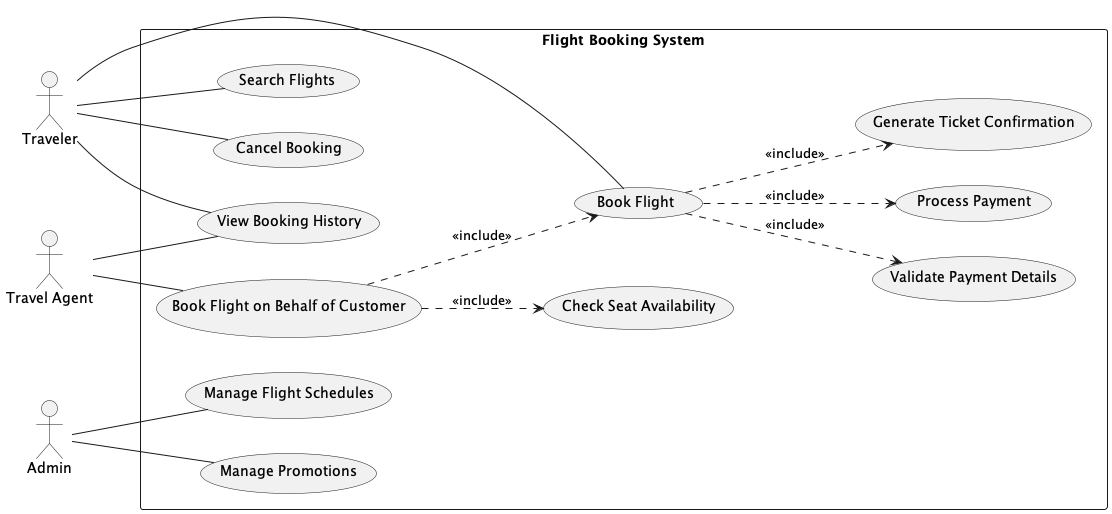
\includegraphics[width=\linewidth]{figures/domain8_antipattern}
    \caption{Antipattern: two FD-include instance groups.}
  \end{subfigure}
  \hfill
  \begin{subfigure}[t]{0.40\textwidth}
    \centering
    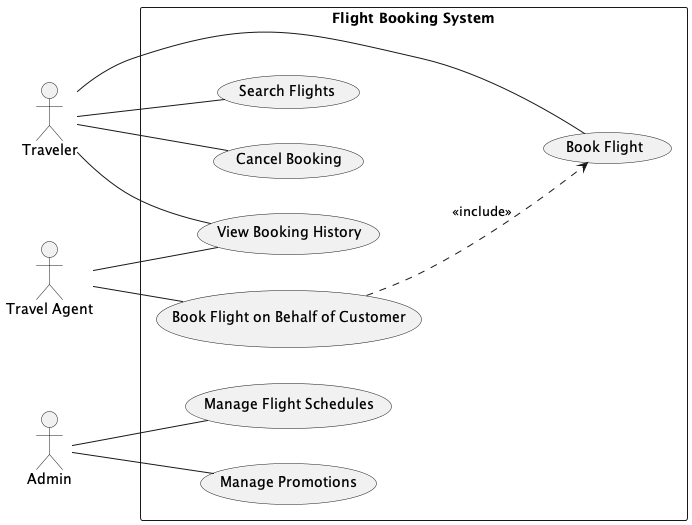
\includegraphics[width=\linewidth]{figures/domain8_refactored}
    \caption{Refactored: all four FD-include instances removed.}
  \end{subfigure}
  \caption{Flight Booking System: antipattern and refactored diagrams.}
  \label{fig:domain8}
\end{figure}

\paragraph{Element definition.}
The system prompt defines a UML \emph{element} as any of four types: actor,
use case, \texttt{<<include>>} arrow, or \texttt{<<extend>>} arrow.  Diagram size is expressed as a total element count,
with the target for each domain drawn from the size tier range.  The two
tiers in Table~\ref{tab:size} are deliberately non-contiguous: small
diagrams contain at most one instance group,
while medium diagrams are large enough to support up to three.  The gap
between the tiers ensures structural distinction is preserved regardless
of minor count deviations, since Claude may add or omit a few elements to
produce a coherent domain model.  The ranges therefore serve as target
guidelines rather than strict constraints.

\begin{table}[h]
\centering
\caption{Diagram size tiers used during generation.}
\label{tab:size}
\begin{tabular}{lcc}
\toprule
\textbf{Size} & \textbf{Element range} & \textbf{Max instance groups} \\
\midrule
small  & 9–13  & 1 \\
medium & 24–30 & 3 \\
\bottomrule
\end{tabular}
\end{table}

\paragraph{Structural validity rules.}
Several rules enforce UML correctness.
Every model must include a system boundary rectangle enclosing all use
cases, with all actors placed outside it.
Every use case in both versions must be associated with at least one
actor; a use case with no actor association is invalid.
Actor-to-use-case associations must be undirected lines, and
\texttt{<<extend>>} arrows must point from the extension use case to the
base use case.

\paragraph{Refactoring scope.}
The system prompt encodes the refactoring strategy supplied in the
antipattern specification.  The refactored
version must be derived strictly from the antipattern version, only
elements that participate in FD-include instances may be removed, and no
new use cases, actors, or associations may be introduced.  This constraint
ensures that the two versions are comparable and that the refactored
version contains no spurious domain enrichment.

\paragraph{Response format.}
The system prompt instructs Claude to produce two PlantUML diagram
versions: one with FD-include instances embedded and one with those
instances refactored away.  It also requires an \emph{antipattern detection label}, a JSON-formatted
structured output recording whether the antipattern is present, which elements are
involved in each instance, and a natural-language explanation.  The schema
is illustrated in Listing~1; refactored versions carry a fixed negative label
(\texttt{"detected": false}, empty \texttt{antipatterns} list).  Each element is identified by its display name followed by its PlantUML identifier in parentheses (e.g.\ \texttt{UC1}), enabling a downstream modeling tool to locate and refactor the specific use case without ambiguity.

\begin{figure}[h]
\begin{lstlisting}[language=json,
  caption={Example antipattern detection label.},
  label={lst:json}]
{
  "detected": true,
  "antipatterns": [{
    "antipattern_name":
      "Functional Decomposition: Using the include relationship",
    "instance_count": 1,
    "instances": [{
      "elements": [
        "Withdraw Cash (UC3)",
        "Validate Account (UC4)"
      ],
      "explanation": "'Validate Account' (UC4) is included by
        'Withdraw Cash' (UC3), has no direct actor association
        ... making it a functional decomposition."
    }]
  }]
}
\end{lstlisting}
\end{figure}

The user prompt is issued once per domain and specifies the target
domain and a target element count drawn from the size tier range.
The Claude Opus 4.6 API is called with
this prompt; the response yields a positive sample (the antipattern PlantUML
source with its detection label) and a negative sample (the refactored
PlantUML source), which are then submitted for manual review.
Once approved, each sample is serialized as a conversational training record
containing three messages: a fixed system prompt, a user message carrying the
PlantUML source, and an assistant message containing the antipattern detection
label.  Listing~\ref{lst:sample} shows a condensed positive sample; the
corresponding negative (refactored) sample is identical in structure but with
\texttt{"detected": false} and an empty \texttt{"antipatterns"} list.

\begin{figure}[H]
\begin{lstlisting}[language=json,
  caption={Condensed positive training sample.},
  label={lst:sample}]
{
  "messages": [
    {
      "role": "system",
      "content": "You are an expert in UML use case diagram analysis..."
    },
    {
      "role": "user",
      "content": "Analyze the following PlantUML use case model and
                  detect if it contains any antipatterns. ......
                  @startuml
                  ......
                  @enduml"
    },
    {
      "role": "assistant",
      "content": "{ detected: true, .......... }"
    }
  ]
}
\end{lstlisting}
\end{figure}

\subsection{Quality Review}
\label{sec:review}

Each generated pair is manually reviewed.  Despite the detailed prompt constraints,
Claude does not always produce fully conformant diagrams; observed issues
include use cases with no actor association, violation of the system
boundary rule, refactored versions that retain FD-include elements or
introduce new use cases absent from the antipattern version, and extension
arrows pointing in the wrong direction.  When issues are found, the
reviewer notes them as free-text descriptions of the specific violations.
Those notes are then passed to Claude as part of the user prompt, asking it
to regenerate the pair while correcting the identified issues.  This loop
typically resolves violations within one or two additional attempts.


% ==============================================================================
\section{Dataset Characteristics}
\label{sec:dataset}

The pipeline produced 194 antipattern/refactored pairs spanning as many distinct
application domains (85 small, 109 medium), yielding 388 training samples in total.
One pair per domain ensures the model generalizes across domain
vocabulary rather than memorising domain-specific patterns.
Table~\ref{tab:stats} summarises the structural properties of the generated
diagrams.

\begin{table}[h]
\centering
\caption{Structural statistics of the generated diagram dataset.}
\label{tab:stats}
\begin{tabular}{lcc}
\toprule
\textbf{Metric} & \textbf{Antipattern} & \textbf{Refactored} \\
\midrule
Samples                           & 194   & 194   \\
\midrule
Total elements (mean)           & 15.3  & 11.4  \\
Use cases (mean)                  & 10.2  & 8.2   \\
Actors (mean)                     & 2.9   & 2.9   \\
Include relationships (mean)      & 2.1   & 0.1   \\
\midrule
Instances per sample (mean)       & 1.96  & —     \\
Instances per sample (range)      & 1–5   & —     \\
\midrule
Diagrams with size \emph{small}   & 85    & 85    \\
Diagrams with size \emph{medium}  & 109   & 109   \\
\bottomrule
\end{tabular}
\end{table}

The difference in mean element count between antipattern (15.3) and
refactored (11.4) versions directly reflects the refactoring: removing
FD-include instances eliminates inclusion use cases and their
\texttt{<<include>>} arrows, reducing total elements by approximately 4 per
diagram on average.  Only 16 of 194 refactored diagrams retain any
\texttt{<<include>>} relationships, confirming that the generation pipeline
correctly preserves only legitimate includes (those whose inclusion
target is associated with an actor or is included by multiple use cases).
The antipattern instance distribution (1--5 instances per diagram) provides
the model with varied label complexity, including cases
where multiple base use cases each decompose into multiple sub-steps.

% ==============================================================================
\section{Fine-Tuning}
\label{sec:finetuning}

We apply parameter-efficient fine-tuning (PEFT) to Qwen2.5-Coder-3B-Instruct~\cite{hui2024qwen2}, a 3B-parameter LLM from the Qwen2.5-Coder series.  Its pretraining corpus includes large quantities of code and structured text, making it well-suited to PlantUML syntax and structured output formatting.  Low-Rank Adaptation (LoRA)~\cite{hu2022lora} adapters are applied to all attention and feed-forward projection matrices with rank $r = 8$ and scaling factor $\alpha = 16$, training 0.48\% of total parameters.  Samples are formatted using the Qwen2.5 chat template with system, user, and assistant turns, with a maximum sequence length of 2048 tokens.  The dataset is split into training and test sets using a domain-stratified 80/20 partition, where entire domains (both antipattern and refactored samples) are assigned to either split, ensuring no domain appears in both.  This yields 155 training domains (310 samples) and 39 test domains (78 samples).  The model is trained for 6 epochs; training loss converged smoothly from above 1.0 to a final value of 0.18, as shown in Figure~\ref{fig:loss}.

\begin{figure}[h]
  \centering
  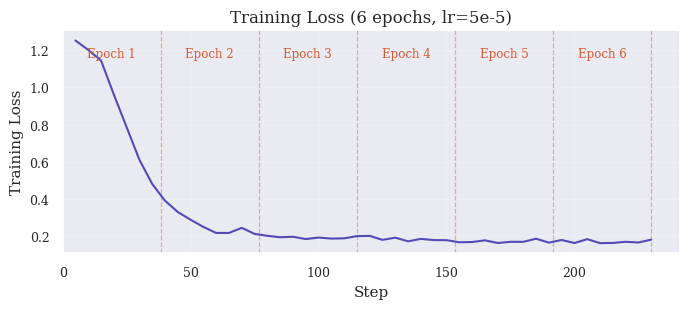
\includegraphics[width=0.85\linewidth]{figures/finetune_loss_curve}
  \caption{Training loss over 6 epochs.}
  \label{fig:loss}
\end{figure}

% ==============================================================================
\section{Evaluation}
\label{sec:evaluation}


Test samples are evaluated at two levels: detection and instance.  Detection
accuracy is the fraction of diagrams for which the model correctly predicts
the \texttt{detected} field of the detection label; for positive predictions,
the antipattern name is also verified.  The model correctly
predicted the presence or absence of an antipattern in 71 of 78 test
diagrams, yielding a detection accuracy of 91.0\%, with the correct
antipattern name predicted in all positive cases.

Instance classification compares the predicted instance list against the
detection label and assigns TP, TN, FP, and FN counts as follows.  A
negative sample (refactored diagram) predicted as negative contributes one
TN; any instance the model predicts on a negative sample contributes one FP.
For a positive sample, each expected instance that the model correctly
predicts contributes one TP, each missed instance contributes one FN, and
each predicted instance with no match in the expected list contributes one
FP.  For example, if a positive sample expects two instances and the model
predicts two but only one matches, the result is 1\,TP, 1\,FP, and 1\,FN.
Matching checks that \texttt{elements} exactly matches the expected list and
that the \texttt{explanation} is semantically correct; all results were manually verified to resolve ambiguous cases.  Precision, recall, F$_1$,
instance classification accuracy, and Matthews Correlation Coefficient (MCC)
are derived from these counts.  Table~\ref{tab:metrics} reports the results
over 128 verified classification outcomes.

\begin{table}[h]
\centering
\caption{Instance classification results over 128 classification outcomes across 78 test samples.}
\label{tab:metrics}
\begin{tabular}{lc}
\toprule
\textbf{Metric} & \textbf{Value} \\
\midrule
True positives  (TP)   & 66    \\
True negatives  (TN)   & 32    \\
False positives (FP)   & 18    \\
False negatives (FN)   & 12    \\
\midrule
Precision               & 0.79 \\
Recall                  & 0.85 \\
F$_1$                   & 0.82 \\
Instance classification accuracy  & 0.77 \\
MCC                     & 0.50 \\
\bottomrule
\end{tabular}
\end{table}

In antipattern detection, recall is the more critical metric, since a missed
antipattern remains silently in the model whereas a false positive can be
dismissed by the modeller on inspection.  The model achieves a recall of 0.85, recovering the majority of expected
FD-include instances, which is the desirable outcome in this context.
Precision at 0.79 reflects some false-positive tendency, as the model
occasionally flags an FD-include instance where none was intended, but this
is an acceptable trade-off.  The MCC of 0.50 confirms a moderate-to-strong
positive correlation between predictions and ground truth, despite the modest
dataset size.

The 12 FNs cluster in medium-size diagrams with 4--5 antipattern instances,
which suggests the model struggles to identify all instances when multiple
base use cases each carry FD-include instances.  The 18 FPs primarily involve
inclusion use cases that are associated with an actor in the diagram.  Both error classes point to the same underlying challenge of comprehensive
structural scanning when instance count is high.

% ==============================================================================
\section{Discussion}
\label{sec:discussion}


The results validate that a frontier LLM can serve as a reliable diagram
labeller, as all generated pairs passed manual review, with violations
corrected through targeted regeneration, and the structural statistics
confirm that refactored versions faithfully remove antipattern elements
without introducing spurious additions (16 out of 194 retain legitimate
includes, consistent with the prompt intent).  The model achieves competitive
detection performance with only 3 billion parameters and $<0.5\%$ of its
weights updated, confirming that synthetic data generation combined with
parameter-efficient fine-tuning enables effective specialisation of a compact
LLM at modest computational cost.


The current dataset targets only FD-include; the full antipattern
catalogue~\cite{elattar2006matching,elattar2010improving} covers many
further types (e.g.\ FD-extend, Accessing an Extension Use Case), and
generalisation to any of these would require repeating the generation and
fine-tuning process, or jointly training on multiple antipatterns
simultaneously.  A second concern is synthetic distribution shift, as Claude Opus exhibits
systematic stylistic preferences that may differ from practitioner-authored
diagrams, so performance on real-world inputs remains to be evaluated.  Generation is also capped at 5 antipattern instance
groups per diagram, whereas real-world diagrams may contain more; the error
analysis already suggests degradation at 4--5 instances.  The model was trained and evaluated exclusively on PlantUML-formatted
diagrams, so its applicability to other use case diagram notations or
modeling tools remains untested.  Finally, 78 test samples across 39 domains
yield somewhat unstable metric estimates, and a larger held-out set would
provide more reliable performance bounds.


Several extensions present themselves naturally. The most immediate is broadening the dataset to cover multiple antipattern types simultaneously, working towards a unified model capable of detecting a full antipattern catalogue. Expanding the diagram size range to include large diagrams (31--54 elements) would stress-test the model on more complex inputs. Evaluating on a hand-crafted benchmark of real practitioner diagrams would measure how well the model generalizes beyond synthetically generated examples. A natural progression of the task is to move from detection to refactoring, where the model not only identifies antipattern instances but also outputs the corrected diagram.

% ==============================================================================
\section{Related Work}
\label{sec:related}


A metric-based approach for antipattern detection in UML designs~\cite{fourati2011metric} targets class and sequence diagrams.
Their approach detects five antipatterns including Functional Decomposition
by computing OO quality metrics such as coupling, cohesion, and complexity,
and comparing them against predefined thresholds.  While it operates at the
UML design level, the approach requires manually defined thresholds.  Our approach differs by learning detection
from examples rather than from metrics or rules, and targets use case diagrams
directly from their PlantUML source.

The most comprehensive catalogue of use case model antipatterns to date~\cite{elattar2010improving} identifies 26 recurring
modeling defects (including FD-include targeted in this work) and codifying them as machine-checkable heuristics within
ARBIUM, a supporting tool.  Detection in ARBIUM is semi-automated via
OCL-style queries; however, refactoring suggestions are made textually and
applied by the developer manually.  Our work draws on their antipattern
taxonomy and takes the next step by replacing the rule-based detector with the model, removing the need for hand-crafted detection rules and
enabling operation on plain-text PlantUML sources without a formal model
repository.

Subsequent work~\cite{khan2016model} extends the ARBIUM line by
automating the refactoring step through model transformations: OCL queries
identify antipattern instances, and ATL transformations then apply the
prescribed structural repairs.  While this fully automates the
detect-and-refactor loop for a subset of the catalogued antipatterns, the
approach still relies on expert-authored formal rules and operates on
structured model repositories rather than textual diagram sources.  Our
approach is complementary: by training an LLM on labeled diagram pairs, we
show that the detection task can be learned from examples alone, without
hand-crafted rules.


Early assessments of ChatGPT's ability to generate UML class diagrams found
syntactic and semantic limitations in models of that era~\cite{camara2023chatgptuml}.
More recent studies show frontier models performing markedly better on
structured diagram generation tasks~\cite{enase26,alsayegh2026stride}.
Our work builds on this capability but uses it for labeled pair
generation rather than description-to-diagram translation.



% ==============================================================================
\section{Conclusion}
\label{sec:conclusion}

We have presented an end-to-end pipeline for fine-tuning an LLM
to detect the Functional Decomposition antipattern in PlantUML use case
diagrams.  The pipeline uses Claude Opus as a synthetic diagram author to
generate 388 high-quality labeled training samples across 194 application
domains, validated through a structured manual review workflow.
Qwen2.5-Coder-3B-Instruct, fine-tuned with LoRA on this dataset, achieves
91.0\% detection accuracy on a domain-held-out test set, demonstrating that
PEFT on LLM-generated synthetic data is an
effective strategy for specializing compact models on structured UML
reasoning tasks.  The pipeline is designed to scale, as additional antipattern
types can be added to the configuration and the generation process repeated,
extending the detector to new antipattern types without any manual data collection.
The dataset, generation scripts, fine-tuning notebook, and evaluation results are
publicly available~\cite{khan2026repo}.

% ==============================================================================
\bibliographystyle{apalike}
\setlength{\bibsep}{4pt}
\bibliography{references}

\end{document}
